\section{Additional Results}
\label{app:results}

\begin{table}[h]
  \centering\small
  \caption{\ours{} (GDN) against the best \emph{strengthened} baseline per regime (same NMPC, front end and input target; only the estimator differs). Gain $=$ median RMSE ratio; one-sided Wilcoxon on 140 paired trials.}
  \label{tab:strong}
  \begin{tabular}{l l r r r}
\toprule
Regime & best strong baseline & GDN gain & wins & $p$ (Wilcoxon) \\
\midrule
Base & MMAE & 0.87$\times$ & 7/140 & 1.00 \\
Gauss.\ noise & robust KF & 1.03$\times$ & 78/140 & $4\!\cdot\!10^{-3}$ \\
Heavy-tail & robust KF & 1.07$\times$ & 83/140 & 0.01 \\
Outliers & robust KF & 1.01$\times$ & 93/140 & $5\!\cdot\!10^{-5}$ \\
Dropout & robust KF & 1.26$\times$ & 117/140 & $<\!10^{-6}$ \\
Rotor flicker & MMAE & 1.50$\times$ & 81/140 & $<\!10^{-6}$ \\
Impacts & robust KF & 0.84$\times$ & 33/140 & 1.00 \\
Stress (all) & robust KF & 1.11$\times$ & 78/140 & $3\!\cdot\!10^{-3}$ \\
\bottomrule
\end{tabular}

\end{table}

\begin{figure}[h]
  \centering
  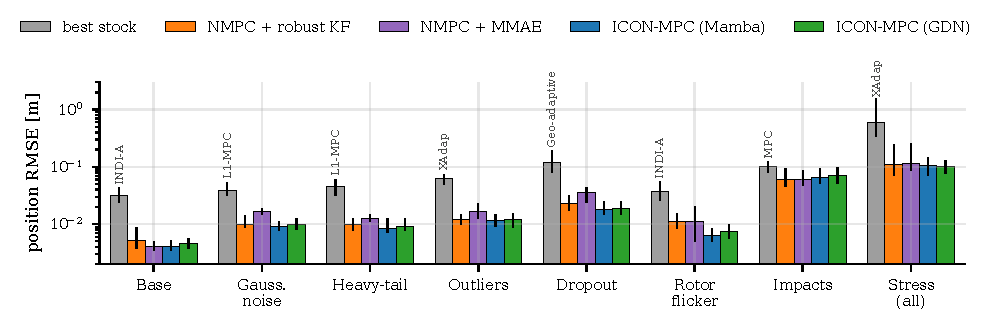
\includegraphics[width=\linewidth]{figures/tracking_results.pdf}
  \vspace{-6mm}
  \caption{Median position RMSE (log scale; whiskers show the inter-quartile range) over 140 paired trials per regime. Grey: best of the seven stock controllers, whose name is shown above the bar. Orange/purple: our strengthened NMPC baselines. Blue/green: \ours{} with Mamba and with GDN estimators.}
  \label{fig:tracking}
\end{figure}

\begin{table}[h]
  \centering\small
  \caption{Obstacle scenarios (140 paired trials each): unsafe-trial rate, median RMSE [cm] and an exact one-sided McNemar test of ``baseline is less safe than \ours{}''.}
  \label{tab:obstacles}
  \begin{tabular}{l rrr rrr}
\toprule
 & \multicolumn{3}{c}{Base (no sensing faults)} & \multicolumn{3}{c}{Stress} \\
\cmidrule(lr){2-4}\cmidrule(lr){5-7}
Controller & unsafe & RMSE & $p$ & unsafe & RMSE & $p$ \\
\midrule
best stock (no constraints) & 100.0\% & 11.8 & $<\!10^{-6}$ & 99.3\% & 17.3 & $<\!10^{-6}$ \\
NMPC nominal + 3 cm & 0.0\% & 10.1 & 1.00 & 22.1\% & 18.8 & $2\!\cdot\!10^{-5}$ \\
NMPC+KF, no margin & 72.9\% & 5.2 & $<\!10^{-6}$ & 68.6\% & 7.2 & $<\!10^{-6}$ \\
NMPC+KF + 3 cm & 0.0\% & 7.6 & 1.00 & 14.3\% & 9.4 & $2\!\cdot\!10^{-3}$ \\
NMPC+KF + ACI & 2.1\% & 5.6 & 0.12 & 12.9\% & 9.2 & $6\!\cdot\!10^{-3}$ \\
NMPC+KF + ACI + 1 cm & 0.0\% & 6.4 & 1.00 & 16.4\% & 10.1 & $2\!\cdot\!10^{-4}$ \\
NMPC+MMAE + 3 cm & 0.0\% & 7.4 & 1.00 & 11.4\% & 12.3 & 0.04 \\
NMPC+MMAE + ACI + 1 cm & 0.0\% & 6.3 & 1.00 & 10.0\% & 12.6 & 0.08 \\
ICON + 3 cm & 0.0\% & 7.5 & 1.00 & 10.0\% & 8.9 & $8\!\cdot\!10^{-3}$ \\
\textbf{ICON + ACI (ours)} & 0.0\% & 6.2 & -- & 5.0\% & 9.2 & -- \\
\bottomrule
\end{tabular}

\end{table}

\paragraph{Ablation and compute.}
Tables~\ref{tab:ablation} and~\ref{tab:compute} support \S\ref{sec:ablation} and the compute paragraph of \S\ref{sec:exp-tracking}.

\begin{table}[h]
  \centering\small
  \caption{Ablation: median RMSE [cm] (140 paired trials per regime; superscript gives the success rate when below 100\%). Upper block: adding components cumulatively. Lower block: removing one component from the full model. All learned rows use training seed 0.}
  \label{tab:ablation}
  \resizebox{\linewidth}{!}{\begin{tabular}{l rrrrrrrr}
\toprule
Variant & Base & Gauss.\ noise & Heavy-tail & Outliers & Dropout & Rotor flicker & Impacts & Stress (all) \\
\midrule
NMPC, nominal model (no drag, no estimator) & 5.08 & 4.89 & 4.98 & 5.08 & 6.08 & 9.45 & 9.52 & 22.72$^{95}$ \\
\quad + rotor-drag model & 4.02 & 4.01 & 3.98 & 4.01 & 5.02 & 8.52 & 8.83 & 20.98$^{94}$ \\
\quad + robust lumped KF & 0.52 & 1.00 & 0.98 & 1.19 & 2.31 & 1.11 & 5.92$^{95}$ & 11.06$^{92}$ \\
\quad + learned estimator: GRU & 0.52 & 1.02 & 1.00 & 1.23 & 1.87 & 0.79 & 6.53 & 9.97$^{98}$ \\
\quad + learned estimator: Mamba & 0.41 & 0.92 & 0.81 & 1.02 & 1.81 & 0.64 & 6.54 & 9.44 \\
\quad + learned estimator: GDN (full) & 0.46 & 0.97 & 0.91 & 1.19 & 1.79 & 0.74 & 7.53 & 9.34$^{98}$ \\
\midrule
full $-$ robust front end & 0.46 & 0.97 & 0.93 & 1.83 & 24.22$^{81}$ & 0.66 & 6.92 & 55.98$^{58}$ \\
full $-$ learned state filter & 0.46 & 0.94 & 0.89 & 1.16 & 1.93 & 0.76 & 7.64 & 9.99$^{99}$ \\
full $-$ offset-free input reference & 0.46 & 0.97 & 0.91 & 1.19 & 1.80 & 0.75 & 7.53 & 9.53$^{99}$ \\
\bottomrule
\end{tabular}
}
\end{table}

\begin{table}[h]
  \centering\small
  \caption{Controller compute per 100\,Hz step (single CPU thread; 30 trials run in parallel) and outcome under stress.}
  \label{tab:compute}
  \begin{tabular}{l r r r r}
\toprule
Controller & mean [ms] & p99 [ms] & stress success & stress RMSE [cm] \\
\midrule
Geometric & 0.42 & 3.3 & 14\% & fail \\
Geo-adaptive & 0.50 & 3.4 & 17\% & fail \\
L1-Geo & 0.63 & 3.7 & 7\% & fail \\
INDI-A & 0.39 & 3.1 & 9\% & fail \\
L1-MPC & 0.54 & 5.5 & 10\% & fail \\
MPC & 0.32 & 3.3 & 59\% & 86.1 \\
XAdap & 0.62 & 5.2 & 73\% & 59.3 \\
\midrule
NMPC + robust KF & 3.59 & 7.4 & 92\% & 11.1 \\
NMPC + MMAE & 4.43 & 9.1 & 96\% & 11.2 \\
\textbf{ICON-MPC (GDN)} & 3.93 & 6.5 & 98\% & 9.3 \\
ICON-MPC (Mamba) & 3.65 & 5.9 & 100\% & 9.4 \\
\bottomrule
\end{tabular}

\end{table}

\paragraph{Training-seed variability.}
Table~\ref{tab:seeds} lists the median RMSE of each training seed. Seed-to-seed variation (up to 15\% under stress) is comparable to the gap between the two selective architectures.

\begin{table}[h]
  \centering\small
  \caption{Median position RMSE [cm] per training seed (140 paired trials per regime).}
  \label{tab:seeds}
  \begin{tabular}{l rrr rrr}
\toprule
 & \multicolumn{3}{c}{GDN seed} & \multicolumn{3}{c}{Mamba seed} \\
\cmidrule(lr){2-4}\cmidrule(lr){5-7}
Regime & 0 & 1 & 2 & 0 & 1 & 2 \\
\midrule
Base & 0.46 & 0.47 & 0.45 & 0.41 & 0.41 & 0.41 \\
Gauss.\ noise & 0.97 & 0.98 & 0.94 & 0.92 & 0.89 & 0.91 \\
Heavy-tail & 0.91 & 0.92 & 0.93 & 0.81 & 0.82 & 0.91 \\
Outliers & 1.19 & 1.18 & 1.14 & 1.02 & 1.13 & 1.13 \\
Dropout & 1.79 & 1.88 & 1.76 & 1.81 & 1.77 & 1.81 \\
Rotor flicker & 0.74 & 0.79 & 0.68 & 0.64 & 0.60 & 0.64 \\
Impacts & 7.53 & 7.07 & 6.65 & 6.54 & 6.53 & 6.48 \\
Stress (all) & 9.34 & 9.76 & 10.30 & 9.44 & 9.37 & 10.77 \\
\bottomrule
\end{tabular}

\end{table}

\paragraph{Qualitative 3D rollouts.}
Figure~\ref{fig:snapshots} shows two stress trials (all faults combined). Animated versions are provided in the supplementary material.

\begin{figure}[h]
  \centering
  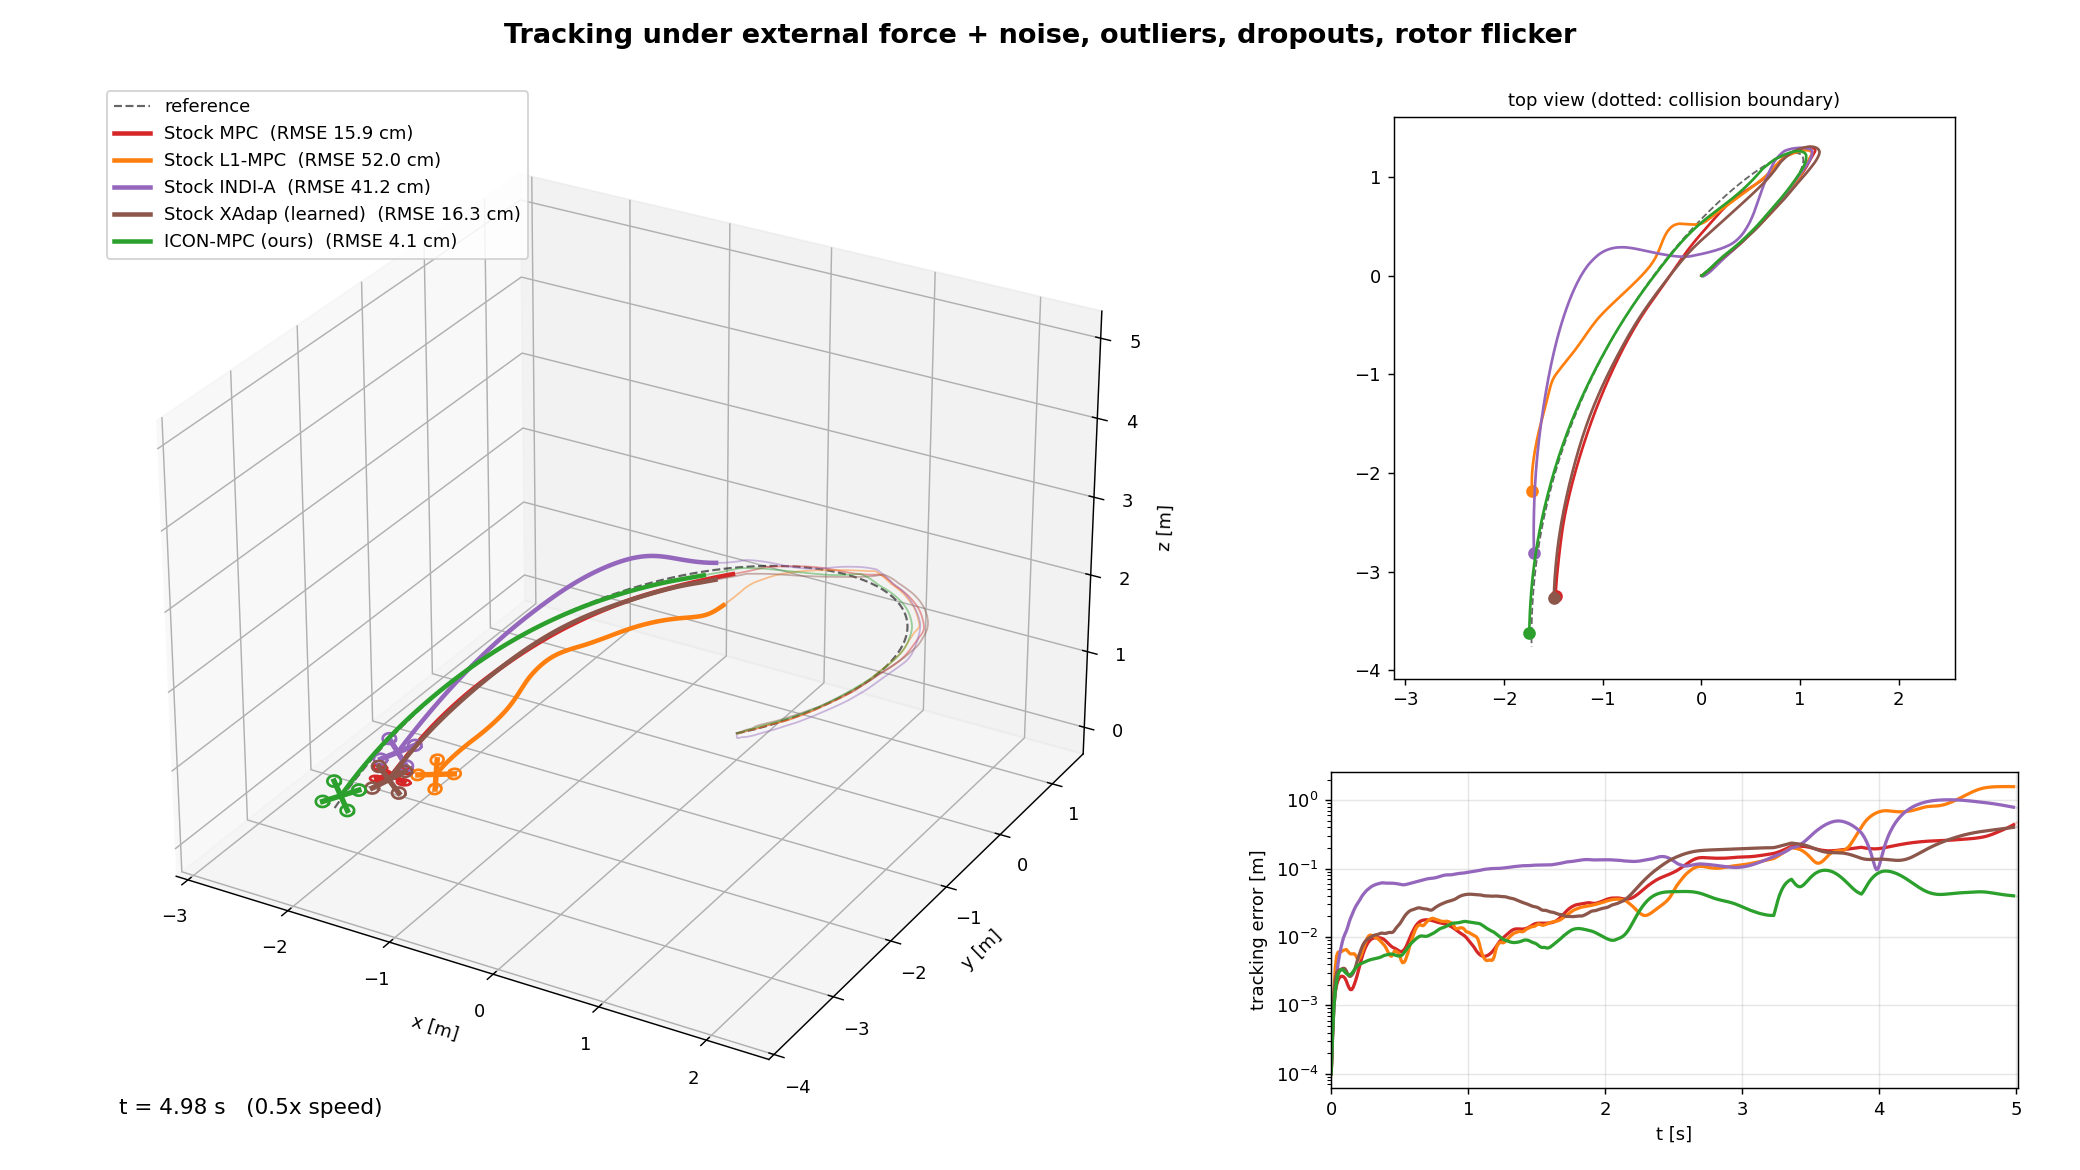
\includegraphics[width=\linewidth]{figures/snapshot_tracking.png}\\[2mm]
  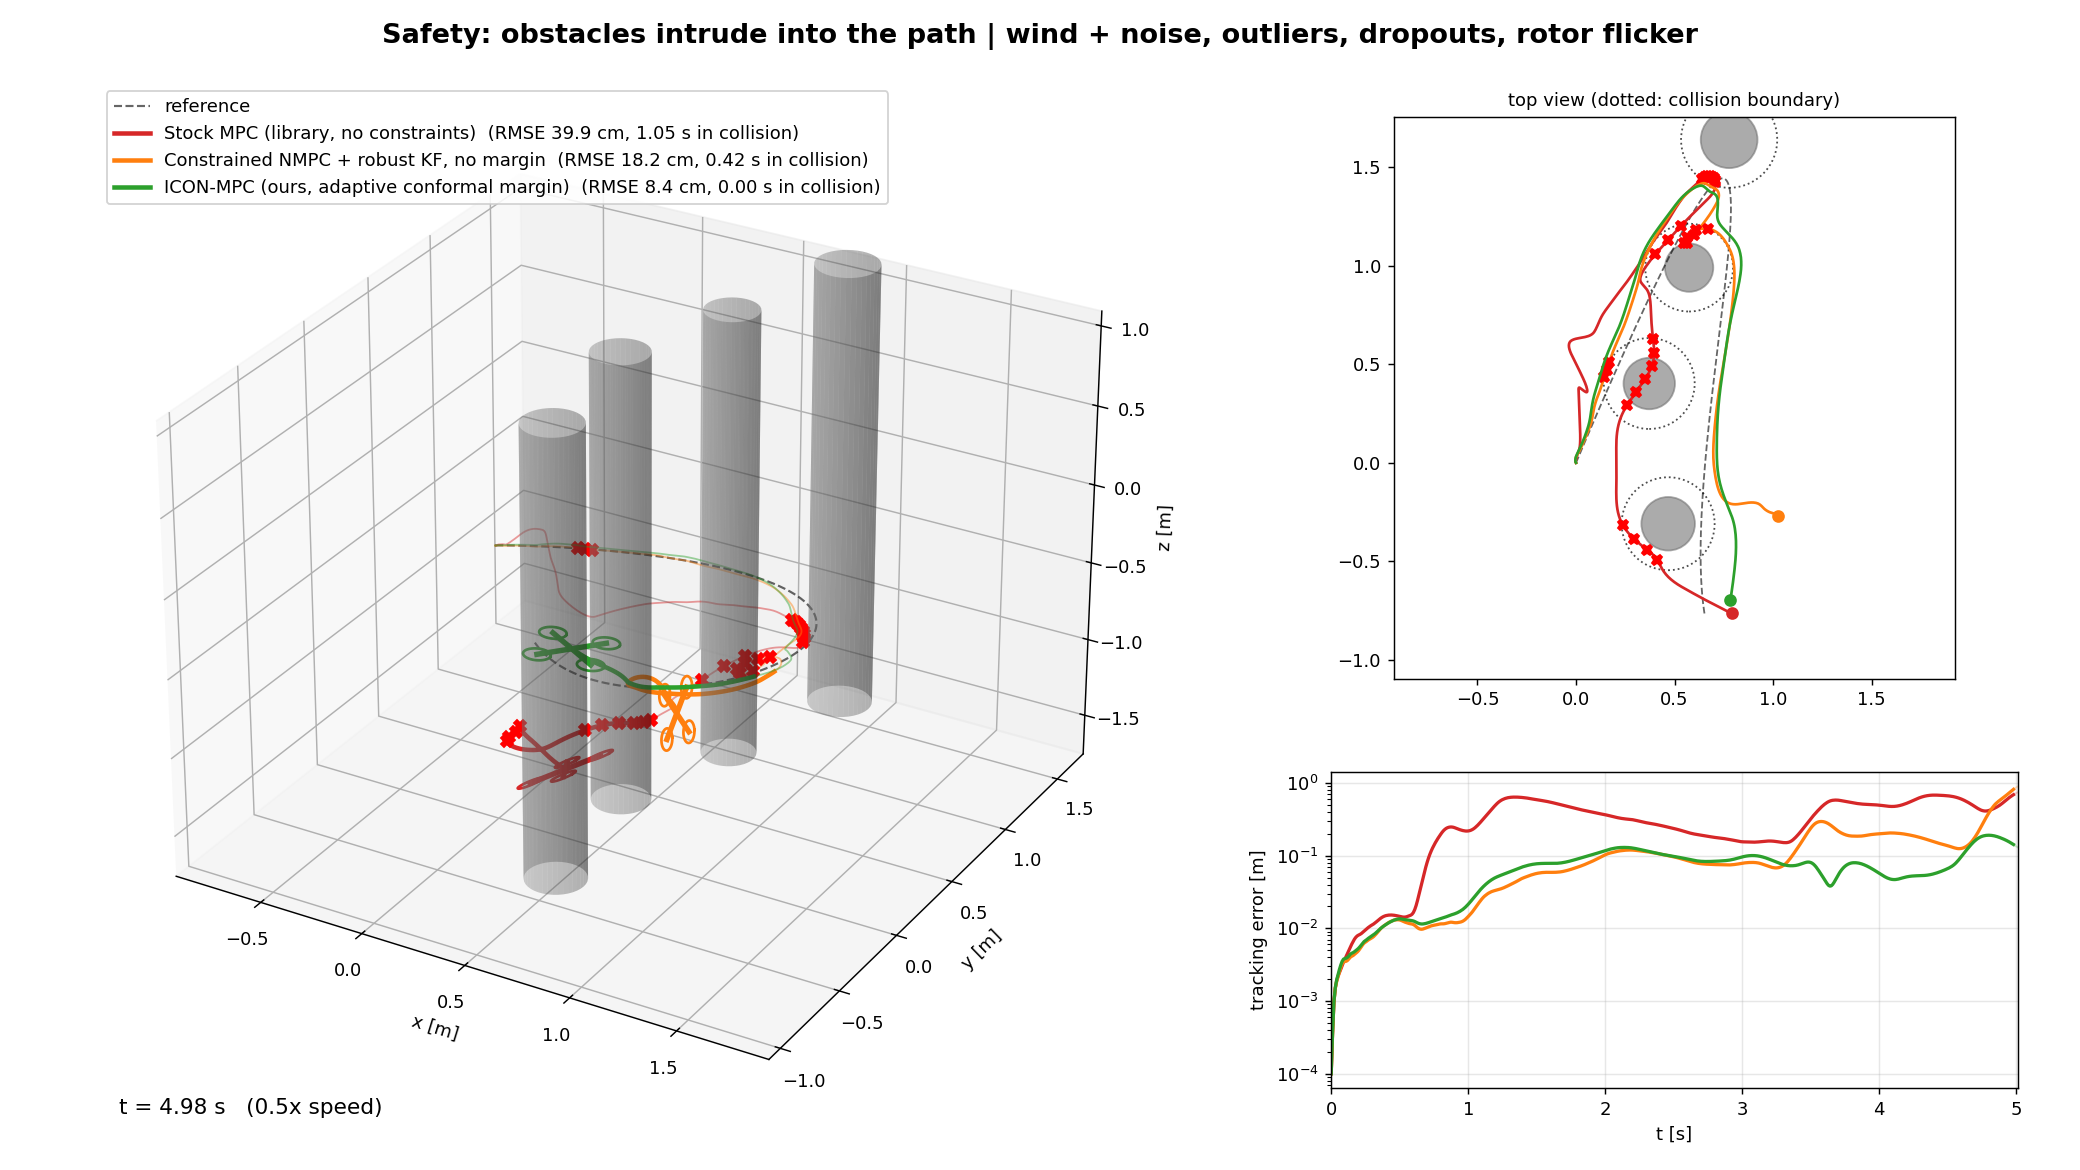
\includegraphics[width=\linewidth]{figures/snapshot_safety.png}
  \caption{\emph{Top:} external force plus stress. \ours{} (green) tracks with 4.1\,cm RMSE, against 15.9--52.0\,cm for the stock MPC, $\mathcal{L}_1$-MPC, INDI-A and XAdap. \emph{Bottom:} wind plus stress, with obstacles intruding into the path (red crosses mark collisions). The stock MPC spends 1.05\,s in collision and the constrained KF-NMPC without a margin 0.42\,s. \ours{} with the conformal margin never collides, with 8.4\,cm RMSE.}
  \label{fig:snapshots}
\end{figure}
